\documentclass[a4paper]{scrartcl}

\usepackage{authblk}

\usepackage[USenglish]{babel}

\usepackage{bibentry}
\usepackage[official]{eurosym}

\usepackage{enumitem}

\usepackage{graphicx}

\usepackage{hyperref}

\usepackage{listings}
\usepackage{minted}

% Font corrections.
\newcommand{\textt}[1]{{\small \texttt{#1}}}

% Disable default paragraph indentation.
\setlength{\parskip}{\baselineskip}
\setlength{\parindent}{0cm}

\title{Modern Ways of Spatial Data Publication}
\author{Wouter Beek ({\small\url{wouter@triply.cc}})}
\author{Laurens Rietveld ({\small\url{laurens@triply.cc}})}
\affil{Triply ({\small\url{http://triply.cc}})}
\date{}

\begin{document}

\maketitle

\begin{abstract}
  Almost every interesting dataset has some spatial component.
  Besides being prevalent, spatial relations -- particularly
  geographical ones -- tie the online to the offline world.  As such,
  they provide a grounding of data stored in databases to the physical
  environment that is described in those databases.

  Given the availability of Semantic Web services, Linked Datasets and
  Open Source web libraries we should be able to build a demontration
  system that allows web programmers to build innovative applications
  on top of integrated Linked (Geo)datasets.  Unfortunately, this is
  not the case.
\end{abstract}

\section{Introduction}

\begin{table}
  \begin{tabular}{|l|l|}
    \hline
    \textbf{Alias} & \textbf{IRI prefix}\\
    \hline
    \hline
    \textt{geo}    & \url{http://www.opengis.net/ont/geosparql#}\\
    \hline
    \textt{bif}    & \url{http://www.openlinksw.com/schemas/bif#}\\
    \hline
    \textt{rdf}    & \url{http://www.w3.org/1999/02/22-rdf-syntax-ns#}\\
    \hline
    \textt{rdfs}   & \url{http://www.w3.org/2000/01/rdf-schema#}\\
    \hline
  \end{tabular}
  \caption{Aliases for commonly occurring IRI prefixes.}
  \label{tab:alias}
\end{table}
  
Earlier research by GeoNovum has resulted in a collection of lessons
learned that describe in great detail the requirements of a modern
spatial data publishing infrastructure.  The purpose of the present
report is to answer the following research question:

\begin{quote}
  How do the lessons learned meet the constraints (e.g. budgets) and
  capabilities (e.g. in-house know-how) of governmental organizations
  on the one hand, and of data users on the other?
\end{quote}


\section{First strategy: use existing tools}

When we started out building our geospatial Linked Data demonstrator
we first did an industry-wide assessment of existing tools.  For this
we have consulted people from multiple domains.  We first determined
the leading query paradigm for geospatial Linked Data: this is
GeoSPARQL~\cite{Battle2011}.  We then determined the tool with the
best GeoSPARQL support: this is Virtuoso\footnote{See
  \url{https://github.com/openlink/virtuoso-opensource}}.  We have
loaded the data into an endpoint hosted at
\url{http://sparql.geonovum.triply.cc/sparql}.

However, even Virtuoso does not support all geometries.  Our data
contains curves, resuting in the following error whenever a curve is
encountered by the query engine:

\begin{lstlisting}
  Virtuoso 42000 Error GEO..: for after check of geo intersects, some
  shape types (e.g., polygon rings and curves) are not yet supported
\end{lstlisting}

Here is an example of a query that gives the above warning (``Pairs of
intersecting geometries that belong to the same resource.''):

\begin{minted}{sparql}
PREFIX geo: <http://www.opengis.net/ont/geosparql#>
SELECT ?y1 ?y2
WHERE {
  ?x geo:asWKT ?y1 .
  ?x geo:asWKT ?y2
  FILTER (bif:st_intersects (?y1, ?y2, 0.1))
}
\end{minted}

A second issue is that some queries do not terminate at all, as
indicated by the following message:

\begin{lstlisting}
  Virtuoso S1T00 Error SR171: Transaction timed out
\end{lstlisting}

An example is an altered version of the above query (``Five pairs of
dissimilar intersecting geometries that belong to the same
resource.''):

\begin{minted}{sparql}
PREFIX geo: <http://www.opengis.net/ont/geosparql#>
SELECT ?y1 ?y2 {
  ?x geo:asWKT ?y1 .
  ?x geo:asWKT ?y2
  FILTER (bif:st_intersects (?y1, ?y2, 0.1) && ?y1 != ?y2)
}
LIMIT 5
\end{minted}

Thirdly, not all combinations of supported functions and supported
shapes are supperted.  For instance, the following implements the geo
query for our original use case:

\begin{minted}{sparql}
PREFIX geo: <http://www.opengis.net/ont/geosparql#>
SELECT ?y (MIN(bif:st_distance(?y, bif:st_point(0, 52))) AS ?z)
WHERE {
  ?x1 geo:asWKT ?y
}
LIMIT 5
\end{minted}

The problem is that distance can only be calculated between points, as
communicated by the following message:

\begin{lstlisting}
Virtuoso 22023 Error GEO..: Function st_distance() expects a geometry
of type 1 as argument 0, not geometry of type 10242
\end{lstlisting}

The fourth and biggest problem is that queries that combine geo
functions and graph relations take \emph{very} long to calculate.  We
have set the limit for query execution to 60 seconds and some queries
still do not succeed within that timeframe.

\begin{lstlisting}
  Virtuoso 42000 Error The estimated execution time 12774 (sec) exceeds the limit of 10000 (sec).
\end{lstlisting}

We have corroborated these results with developers on the Linked Data
Platform team (Kadaster).  They are also deploying geospatial data for
web users and they also discovered that existing triple stores are
unable to support this.


\section{Users have different needs \& capacities (lesson 1)}

In this research project we have tried to address multiple groups of
users by offering result set formats that they are most likely to be
familiar with.  Our demonstrator exposes the following result set
formats:

\begin{itemize}

\item GeoJSON

\item JSON-LD 1.0

\item N-Quads 1.1, N-Triples 1.1

\end{itemize}

The N-Quads and N-Triples formats are, implementation-wise, the
simplest RDF serialization formats available.  They are supported by
almost every RDF processor.  Additional RDF serialization formats like
Turtle 1.1, RDF/XML 1.1 and TRiG 1.1 are also available in ClioPatria.
It would be a low-cost effort to expose them as well.  We notice that
the JavaScript RDF libraries that are currently being developed for
client-side processing do not support, and will maybe never support,
RDF/XML.

RDF JavaScript Libraries Group

https://www.w3.org/community/rdfjs/


\subsection{Header Dictionary Triples (HDT)}
\label{sec:hdt}

Another format that could be added is Header Dictionary Triples
(HDT)~\cite{Fernandez2012} files.  These are currently used to power
the Graph API.  They are also used to power Linked Data Fragments
(LDF)~\cite{Verborgh2014} and the LOD~Laundromat~\cite{Beek2014}.
This format could be interesting for users who want to gather very
large result sets.

Textual serialization formats work well for small results sets.  For
instance, if someone asks the ten nearest monuments then this can
easily be returned in a text description.  However, if someone has a
larger-scale use case one may want to retrieve thousands of results.
For instance someone may request all monuments in The Netherlands in
order to generate a `heat map' of areas with the most monuments.  The
result set of this will be hundreds of megabytes of textual data.  The
users will not be able to process this data off-hand, but would need
to load this in her own database.

TODO


\subsection{GeoJSON}
\label{sec:geojson}

The GeoJSON format is not yet fully standardized.\footnote{GeoJSON is
  a proposed RFC standard as of August 2016.}  The GeoJSON
RFC~\cite{rfc7946} is not a standard in the traditional sense of the
word: a definition of all and only GeoJSON constructs and their
meaning.  For instance, the current RFC does not give a format grammar
but only examples of GeoJSON in use.

It is not very difficult to implement GeoJSON, which is a very
flexible format that can easily be combine with other JSON formats.
Specifically, we were interested in mixing GeoJSON into JSON-LD
constructs.  Some people have worked on this in 2015 under the name
`geojson-ld'\footnote{See
  \url{https://github.com/geojson/geojson-ld}}, but development in
that direction has stalled.

The biggest hurdle towards integrating GeoJSON and JSON-LD into one
format is that JSON arrays are used in JSON-LD for abbreviated object
term notation.  However, GeoJSON uses JSON arrays to represent
geometries (nested lists of floating point coordinates).
This point will be addressed in JSON-LD 1.1\footnote{See \url{https://github.com/json-ld/json-ld.org/issues/397}}.


\subsection{JSON-LD}
\label{sec:jsonld}

JSON-LD 1.0 support was the most problematic to implement.  It differs
from other RDF serializations in that it does not translate a graph to
a sequence of characters (i.e., a proper serialization), but it
instead performs transformations between RDF graphs and JSON trees.
As such it has to merry requirement from both paradigms.  In this
sense JSON-LD is similar to RDF/XML which is already relatively
complex when compared to the N3-family of serializations (N3, Turtle,
TRiG, N-Quads and N-Triples).

There are currently implementations for C\#, Go, Java, Javascript,
PHP, Python, Ruby.  Most notably support for C and C++, languages in
which very many low-level database systems are written, is currently
missing.  Illustratively, one of the most widely used C++-based RDF
processors, Raptor (\url{http://librdf.org/raptor/}) says on its web
site:

\begin{quote}
  JSON-LD is not supported - too complex to implement.
\end{quote}

Virtuoso does not support loading JSON-LD files\footnote{See
  \url{https://github.com/openlink/virtuoso-opensource/issues/478}}
and ClioPatria does not support JSON-LD out-of-the-box either.  We
have written a partial implementation for generating JSON-LD and
included it into library plRdf\footnote{See
  \url{https://github.com/wouterbeek/plRdf/blob/master/prolog/jsonld/jsonld_build.pl}}.


\subsection{OGC standards (GML, WFS, WMS)}

While GeoJSON addresses users from the web and geo domain, it may not
address more advanced GIS users who may want to use more comprehensive
formats standardized by the OGC, such as GML, WFS and WMS.  The cost
of integrating these OGC formats into a Linked Data platform are
considerable, because they have their own vocabularies that need to be
mapped to and from RDF.  The OGC and W3C are currently working on this
integration in the Spatial Data on the Web Working Group\footnote{See
  \url{https://www.w3.org/2015/spatial/wiki/Main_Page}}.  It is
probalby wise to wait until that WG has come up with a first
(proposed) standard.


\subsection{Findability (lesson 1a)}

One of the most difficult things for web programmers, when confronted
with the system, is to find out \emph{what is in the data}.  For
existing web services this is usually not an issue: there is a limited
numeber of entity types and relations that can be queries.  For
instance, a product review site has users who write reviews for
products.  Products may have companies producing them and users may
themself have ratings.  That's about it.

Linked Data is very different: the monument dataset that we started
out with contains over a hundred unique relationships between entites
belonging to dozens of different types.  And this is only one dataset.
It is inherently impossible to provide a overview of what is in a
large collection of Linked Data, in the same way in which it is
impossible to provide an overview of what is in a large collection of
the web.  What we can do is come up with smart data visualization
techniques.  We found out that no such techniques are currently
available.

Datasets can be very large, so good search functions are required to
let users find the needle in the haystack.

Why

Different users need different information, for example a user who is
interested in locations of bicycle stands, does not need a map with
both bicycle stands and trees on it.  If you allow users to search
through dataset based on space, time and theme, data is better
retrievable.

A user-friendly web service enabling users to easily and intuitively
search and find data.

Provide good search functions, for example let users search for whole
datasets or single objects based on space, time and theme (keyword or
category).


\section{Keep it simple (lesson 1B)}

A platform that enables to easily upload and publish spatial data
sets.

For example, do not ask users to fill in a coordinate reference system
(CRS) when they upload a spatial data set. Generally, the CRS can be
detected from the CRS embedded in the file.

\subsection{Uniform representation of geodata}

\begin{minted}{turtle}
  entitiy:x geosparql:defaultGeometry _:a .
  _:a       geosparql:asWKT "POINT(5.46 51.35)"  ;
            rdf:type geosparql:Geometry     .
\end{minted}

We believe that the above three statements can be rewritten to a
single statement conveying the same meaning:

\begin{minted}{turtle}
  entity:x def:geometry "POINT(5.46 51.35)"^^def:point .
\end{minted}

Our version has the following benefits:

\begin{itemize}

\item No introduction of unnecessary blank node terms.

\item More explicit type information of the kind of geometry (a point
  in this case).

\end{itemize}

These properties result in direct usability imporvements:

\begin{itemize}
  
\item One less level of nestingsimplifies querying.  For instance, we
  need one LDF request to retrieve the geometry of an entity instead
  of two.

\item We can query for geometries of a specific type without having to
  parse geometry values.  For instance, for one of our map views we
  wanted to show polygons but not points and lines.  We achieved this
  with the query%~\ref{lst:datatype}.

\end{itemize}

\begin{minted}{sparql}
  ?e <def/geometry> ?g FILTER (datatype(?g) = <def/polygon>)
  \label{lst:datatype}
\end{minted}


\subsection{Who is allowed to do what (lesson 1c)}

All our data was published as Linked Open Data with no authentication.
In general we notice that Linked Data is far more often \emph{read}
than \emph{written}.  Our demonstration system does allow SPARQL
Update requests to be sent, but we have not advertised or used this
functionalty within the current research.


\subsection{Each speaks its own language and lives in his own world}


\section{Linking (lesson 2b)}

\subsection{Internal links: within datasets}

Geodata, as it is currently published, does not contain explicit
links.  Links can be inferred from implicit cues by human domain
experts, but not by automated and domain-independent means.

The same value sometimes denotes the same thing.  E.g., `Appingedam'
denotes a municipality.  However, Appingedam is sometimes denoted by
`GM0003' (gemeentecode) and occurrences of the same string can denote
different things (e.g., the area of Appingedam changes over time, the
municipality of Appingedam is more than just the area of Appingedam,
and a tourist uses `Appingedam' to denote the center of Appingedam).

The same is true for other value types, e.g., `1903' may denote a year
in the Gregorian calendar or the length of a road in meters.  


\subsection{Value unpacking}

A single value in the source dataset may describe multiple entities
and relations between them.  For instance the small `buurtcode' string
\textt{BU00030002} denotes three entities and two spatial containment
relations:

\begin{minted}{turtle}
  buurt:00030002 rdf:type        def:Buurt      .
  gemeente:0003  geof:sfContains wijk:000300    ;
                 rdf:type        def:Gemeente   .
  wijk:000300    geof:sfContains buurt:00030002 ;
                 rdf:type        def:Wijk       .
\end{minted}

We call the conversion of a simple value to multiple entities and
relations `value unpacking'.  Domain experts have `packed' meaning
into encodings like \texttt{BU00030002}.  Non-domain experts and
machines cannot `see' the meaning that is inside the package.  In
order to make the meaning widely available we must `unpack' it using a
grammar.  For the above code we have to construct the following
grammar.\footnote{The grammar is written in Augmented Backus-Naur Form
  (ABNF), \cite{abnf}.}

\begin{minted}{abnf}
buurt         := "BU" gemeente-code wijk-code buurt-code
buurt-code    := DIGIT DIGIT
gemeente      := "GM" gemeente-code
gemeente-code := DIGIT DIGIT DIGIT DIGIT
wijk          := "WK" gemeente-code wijk-code(Wijk).
wijk-code     := DIGIT DIGIT
\end{minted}

When loading the data we have to tell the machine to \emph{parse}
values within a given column, tag or key using the above grammar.  The
machine is then able to automatically construct the encoded entities
and relations for all such values.

Notice that the above has to be done for every column, tag or key.
Moreover, not all values can be parsed in this way.  For instance,
human language can generally not be parsed by a machine processor.


\subsection{Value enrichment}

Besides combining and splitting values, we sometimes find that a value
is incomplete: it does not contain all the information we need in
order to interpret it.

For instance, very many values are encoded in human languages.  In
order to do anything useful with these values we must at least know to
which language they belong.  For this we run automatic language
detection algorithms on the values.  The accuracy for medium-length
strings is known to be very high (Figure~\ref{fig:natlang}

\begin{figure}
  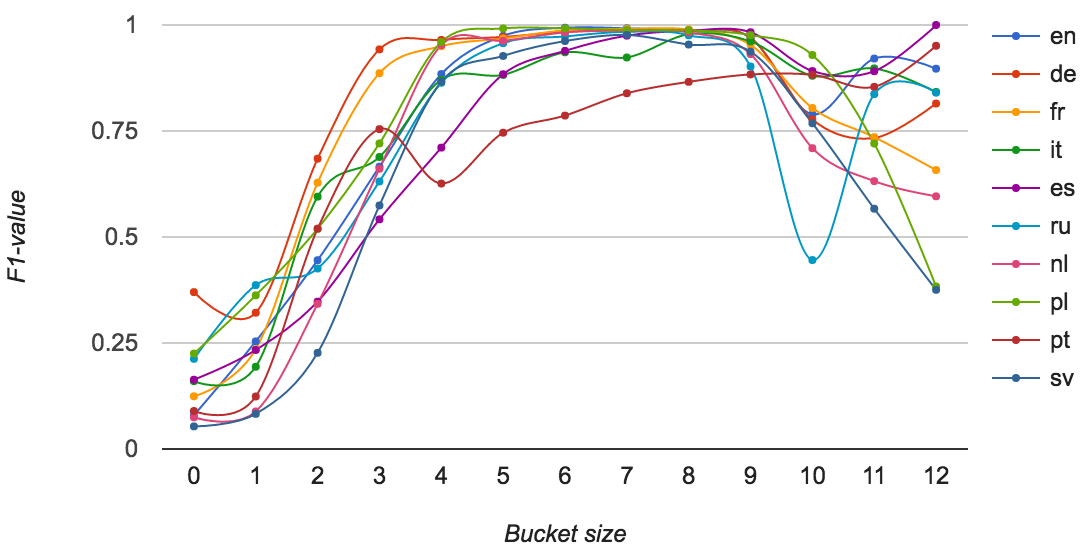
\includegraphics[width=\linewidth]{img/natlang.png}
  \caption{Accuracy of natural language detection in RDF strings for
    the 10 most frequent languages.  Strings of similar lenght are
    combined in buckets.  The size of buckets increases
    logarithmically.  Figure taken from~\cite{Beek2016}.}
  \label{fig:natlang}
\end{figure}

The main benefit of running natural language detection on the current
data collection is to distinguish between Dutch and English strings.


\subsection{Value combining}

For example events are often described with a day, month and/or year
column, tag or key:

\begin{lstlisting}
  <EVENT-ID> | 1997 | Aug | 7
\end{lstlisting}

In order for dates to be comparable with one another they have to be
converted to values of XML Schema Part 2: Datatypes 1.1~\cite{xsd11}.
Month names can be converted using a simple, one-to-one grammar
(Section~\ref{sec:grammar}).  After that values can be converted
manually to datatypes.

\begin{minted}{turtle}
  event:x def:day   "07"^^xsd:gDay    ;
          def:jaar  "1997"^^xsd:gYear ;
          def:maand "8"^^xsd:gMonth   .
\end{minted}

Values can now be automatically combined into the following more
complex datatype:

\begin{minted}{turtle}
  event:x def:date "1997-08-07"^^xsd:date .
\end{minted}

Because support for XML Schema Datatypes is very good overall, dates,
times, durations, lengths, weights, etc. can now be compared through
built-in functions.  For instance the function
\textt{op:dateTime-less-than} is used by SPARQL 1.1 implementations to
directly compare an event to all events that happended before
it~\cite{xquery10}.


\subsection{Persistent IRIs (lesson 2c)}

It is very difficult to ensure persistent IRIs.

Most datasets have no IRIs at all, so we have to mint IRIs for each
entity.  While enriching the data (Section~\ref{sec:enrichment}) the
number of entities increases.  These requires IRIs as well.

We have found the Dutch Linked Data URI strategy to be very beneficial
during this process.  It distinguishes between IRIs for instance
(ABOX) and schema (TBOX) entities.

Publish data in registries at unique persistent URIs to ensure links between data sets are available, attainable and sustainable in the future.

Why

Using URIs, you can link to something in a unique way and therefore uniquely distinguished. You need to use stable HTTP URIs for spatial objects and datasets in order to keep the links future-proof and reliable.
Intended outcome

Registries, and especially the base registries, have proper uri management. Records are made available on a unique persistent uri, which enables the linking of objects within these registries to each other.
Possible approach

Publishing data records on unique persistent URIs requires a URI strategy. For example using the Dutch Linked Data URI Strategy:

URI:

    /id/{resource} 303 redirect to /doc/{resource}
    /doc/{resource}

Example: https://geo4web.apiwise.nl/gemeente/GM0307

URI CBS Amersfoort
How to test

Several flavors exist but we recommend to the use Dutch URI Strategy as it was indexed by Google relatively fast. Read more here 



\section{Motivation for applying for this research topic}

Triply applies for this research topic because it sees innovation
potential for the way geodata is currently published on the Web of
Data.  Triply wants to explore and concretely deliver significant
improvements to the way in which geodata is disseminated to data
consumers.  Triply believes that it is possible to unlock innovation
potential within this tender given (1) the close collaboration with
Geonovum, (2) the presense of other data suppliers such as PDOK and
cultural heritage organizations, and (3) the lessons learned during
the previous tender round on which we can build.

When we look at contemporary geodata publishing practices we see two
worlds colliding: On the one hand there are data publishers that use
OGC standards that are very expressive but also very complex.  On the
other hand there is the Web of heterogeneous and distributed data
sources.  There is a large number of (potential) data consumers that
are using the contemporary Web stack and are used to far simpler and
more Open Web APIs.  (These are the two parties that are also
identified in the research question for this research task.)

Luckily, usability and complexity need not exclude each another once
the Linked Data approach is applied correctly.  Since Linked Data does
not require a single database schema to operate, we have the ability
to disseminate the same data through different but complementary
vocabularies.  For instance, there can be two schemas: one complex and
difficult and antoher simplistic and easy (lesson 1B).  In this
example the two vocabularies cater towards the aforementioned two user
groups.  In this way the same data can be delivered in different ways,
benefitting different groups (lesson 1).  While the specification of
multiple vocabularies/schemas on top of the same data collection comes
at a low cost it does provide the necessary tuning to user
capabilities (lesson 1D).

The other part of the research question targets the ``constraints
(budgets) and capabilities (in-house know-how)'' at the data publisher
side.  Operating costs can be split into fixed and variable costs.
The \textbf{fixed cost} of deploying a Linked Data solution (e.g. a
remotely accessible triple store) is considerable.  At the moment
governmental organizations wish to use and/or provide a Linked Data
deployment they oftentimes have in-house people that do a considerable
portion of the engineering.  There is no clear reason why Linked Data
deployment should require more in-house knowledge then using the
electric grid.  With the Triply Linked Data product a (governmental)
organization uses the Triply Linked Data infrastructure in a similar
way in which it uses the electric grid; it simply connects.  Because
Triply significantly reduces the fixed cost of deploying a Linked Data
solution, the (governmental) organization can focus on curating the
data and extracting value from it.

The \textbf{variable cost} of deploying a Linked Data solution is an
entirely different story.  While it is somewhat difficult to set up a
triple store it is virtually impossible to build one that scales to
service a large amount of (consecutive) users.  When we look at the
SPARQL endpoint observatory SPARQLes ({\small
  \url{http://sparqles.ai.wu.ac.at}})~[\cite{BuildAranda2013}], we see
that 80\% of current SPARQL endpoints have low availability.  When we
look at the 20\% SPARQL endpoints with high availability, we see that
they enforce restrictions on the kinds of questions that can be asked
and the size of answer sets that are returned.  This effectively means
that remote triple stores are either unailable or severely
constrained.  No Web programmer wants to program against a database
with either of these properties.  Triply is the first Linked Data
solution that allows the number of (consecutive) users to scale
without blowing up the variable cost of endpoint operation.  Triply is
able to do this because Triply is based on recent innocations in
large-scale and scalable Linked Data deloyments: Linked Data Fragments
(LDF)~[\cite{Verborgh2014}], Header Dictionary Triples
(HDT)~[\cite{Fernandez2013}] and LOD Laundromat~[\cite{Beek2014}].

\section{Plan of approach}

The plan of approach focuses on realizing maximal impact within a
short period of time.  All crucial decisions in the plan of approach
will be made by Triply's CTO who has extensive experience with
building large-scale data systems.  Some of the low level tasks in the
plan of approach will be performed by a Triply engineer.

\subsection{Requirements analysis}

Triply will collaborate with Geonovum, data providers and task 2
partners in order to make a requirements analysis that specifies what
is needed in order to support the goals of the overarching tender
call.  Making the requirements analysis a shared responsibility will
ensure that development of the demonstrator will be demand-driven.

\subsection{Data conversion and cleaning}

Since some data may either not yet be formatted as RDF or may not yet
be fully standards-compliant, Triply will perform data conversion and
cleaning steps in order to ensure that all data meets certain quality
criteria.  Inherent bugs in the data that cannot be fixed by
technological means alone will be communicated back to the original
data suppliers.

\subsection{Database layer}

The result of the data conversion and cleaning steps will be populated
into a SotA database backend.  The backend will be chosen so as to be
able to service at least one thousand simultaneous API users.  The
focus is here on features that Web developers find beneficial, i.e.,
prioritizing scalability, efficiency and performance (lesson 1B).

\subsection{API layer}

Triply will define and implement a RESTful Web API that follows the
lessons learned, together with formal and de facto standards in Web
API construction.  This RESTful API layer will focus on lowering the
barrier for (Web) programmers to use Geodata.  In line with lesson 3A,
content negotiation will be used to let a data consumer specify the
format s/he prefers.

%Since the Web programmer wants to build an application quickly and
%may not know each and every technology out there, Triply will ensure
%that data can be accessed in each of the currently standardized
%Linked Open Data formats: RDF/XML, N-Triples, N-Quads, TriG, JSON-LD,
%RDFa, Schema.org, IRI dereferencing, Linked Data Fragments (LDF),
%Linked Data Platform (LDP), SPARQL and GeoSPARQL.

%Following lesson 3A this will be done (1) terms of HTTP Accept
%headers and (2) in terms of content-specific URIs (to the extent that
%this does not conflict with the URI persistency requirement).

\subsection{Iteration cycle}

Once the whole system is fully functional and has task 2 partners
programming against it, Triply will assess which changes are needed in
each of the layers in order to improve the demonstrator for maximal
utility.

\section{Results}

This section enumerates the results that will be made available.

\subsection{Data}

Triply will make all cleaned, converted, linked and otherwise enriched
data available to the original data suppliers.  The data will contain
future-proof persistent URIs (lesson 2C) and will contain structured
annotations that make it easy to find when published online (lesson
2D).  Persistent URIs will be based on the Dutch Linked Data URI
Strategy~\cite{Overbeek2013}.

\subsection{Vocabulary}

Triply will make the vocabulary that bridges the geodata and Web API
communities available to Geonovum and/or the original data suppliers.

\subsection{Demonstrator}

Triply will provide a demonstrator Web Service that will be used by
task 2 collaborators.  Data in the demonstrator will be supplied in
standardized Linked Open Data formats (lesson 3A).

\subsection{Reports}

Triply will write a report in which it will validate the lessons
learned with respect to the practice of making large quantities of
geodata available in a Web- and developer-friendly way.

\subsection{Dissemination}

Finally, Triply will communicate the results obtained within the
Geonovum tender with the wider Linked Open Data, Geodata and Web API
communities.  Concretely, Triply will perform the following
dissemination activities:

\begin{enumerate}[noitemsep,nolistsep]
  
\item Triply will, in collaboration with partners, present the results
  of the Geonovum tender at community events about Linked Open Data,
  Geodata, and Geo-oriented Web APIs.
  
\item Triply will write a report describing the tasks that have been
  performed.  The report will also contain the findings and answers to
  the task description questions (as enumerated in the ``Invitation to
  tender'' document).

\item Triply will take the lead in writing a white paper about the
  requirements for the deployment of a scalable Linked Geodata backend
  and an approachable Web API for Open Geodata.  The paper will be
  written in close collaboration with the various partners and will be
  submitted to an appropriate venue (e.g., WWW, ESWC Industry Track or
  Semantics).
  
\end{enumerate}


\subsection{References}

Triply is a startup that is based on research previously conducted by
the Knowledge Representation and Reasoning (KR\&R) group at VU
University Amsterdam (VUA).  Headed by Prof. Dr. Frank van Harmelen,
this is the top research group in the world in the area of Semantic
Web and Linked Data research.

The founders of Triply have proven their ability to \textbf{conduct
  outstanding research} in the field of Semantic Web and Linked Data.
This has resulted in multiple highly cited research papers over the
last two years alone.  The Triply founder's research effort has
culminating in winning the Best Research Paper Award at the
International Semantic Web Conference (ISWC) 2015, which is the top
venue for Semantic Web research.  Here follows a selection of relevant
publications over the last two years:

In addition to delivering outstanding research, the founders of Triply
have proven their ability to \textbf{build outstanding Linked Data
  solutions} as well.  Firstly, the LOD Laundromat
(\url{http://lodlaundromat.org}) ecosystem has won the Best Dutch
Linked Open Data Award 2015 (and ended $3^{rd}$ in the European
competition).  LOD Laundromat is widely recognized as a Game Changer
within the Semantic Web research community.  Secondly, Triply’s CTO
has build Yasgui (\url{http://yasgui.org}), the most feature-rich
SPARQL editor.  Yasgui is used by many high-impact Linked Data
projects and parties such as Sesame, Jena, Smithsonian Museum, German
National Library of Economics and Linked Open Vocabularies.  Thirdly,
Triply’s CEO is involved in the development of the ClioPatria triple
store (\url{http://cliopatria.swi-prolog.org}) and SWI-Prolog’s
Semantic Web library (\url{http://www.swi-prolog.org}).  Finally, the
founders of Triply have recently been involved in the construction of
LOTUS (\url{http://lotus.lodlaundromat.org/}), a large-scale and
customizable Semantic Web search engine.


\subsection{Indication of in-kind investment}

Triply will match Geonovum’s investment amount with an in-kind
investment of equal size, i.e., \euro{}10.000,- The in-kind investment
is necessary to realize the ambitions expressed in the plan of
approach.


\subsection{Statement of agreement}

Triply agrees to publish all research results and deliverables that
flow from this tender under the CC/by license.


\section{Quantifying the effort}

There were also some `hidden costs', i.e., either things that we
expected to be very simple but that turned out to be very difficult,
or things that we did not expect in the first place.

Firstly, we had to spend an enormous amount of time converting the
various data formats (Section~\ref{sec:conversion}).  After the
conversion, we had to go through several iterations of transforming
the data to improve its quality.  While our transformed data has a
much higher quality than the source data we started out with, we
believe that there are still several more iterations needed to get the
data to a quality level that allows generic (SPARQL) queries to be
performed painlessly (i.e., without ad-hoc string manipulation).

Secondly, we expected to find a plethora of tools that allow Linked
Data to be exposed to web programmers.  After all, Linked Data is web
data.  We were very surprised to find that this is not the case at
all.  In fact, there were many perfectly valid requests by the web
programmers we worked with that could not be easily implemented by
integrating some existing library.


\section{Conclusion}

We conclude that it is not yet possible to go from a loose collection
of (geo)data sources to a usable web service for web programmers
within two months.  There are too many missing pieces and the cost of
data conversion and transformation is simply too high.

However, we do believe that the lessons learned in previous research
and validated in our research do point to a.





\bibliographystyle{plain}
\bibliography{main}

\end{document}
